\subsection{CDC tracking}
The CDC tracking was performed in uniform magnetic field, so its track is helix track which was introduced by K.Fuji\cite{helix} as following equations.
\begin{eqnarray}
  x(\phi)=d_{\rho}\cos\phi_0+\frac{1}{\rho}(\cos\phi_0-\cos(\phi_0+\phi)\\
  y(\phi)=d_{\rho}\sin\phi_0+\frac{1}{\rho}(\sin\phi_0-\sin(\phi_0+\phi)\\
  z(\phi)=d_z-\frac{1}{\rho}\tan\lambda \dot \phi
\end{eqnarray}
where $d_{\rho}$ is the distance of the helix from the origin point in the $xy$ plane, $d_z$ is distance of $z$ direction, $\phi_0$ is the azimuthal angle to $z$-axis, $\lambda$ is elevation angle
and $\rho$ is the inverse of the radius of the helix.\\
In this parametrization, charged particle momentum is represented as below,
\begin{equation}
  \bm{p}=\frac{cB}{\rho}\left(
  \begin{array}{c}
    -\sin(\phi_0+\phi) \\
    \cos(\phi_0+\phi) \\
    \tan\lambda
  \end{array} \right)
\end{equation}
where c is the light velocity, B is strength of uniform magnetic field in the $z$ direction.

Drift time convert to drift length using fifth order polynomial function which function was iteratively adjusted to minimize systematic shift.
Fig\ref{fig:CDC_dl_dt} shows drift time and drift length.

\begin{figure}[htbp]
  \begin{tabular}{cc}
    \begin{minipage}{0.5\hsize}
      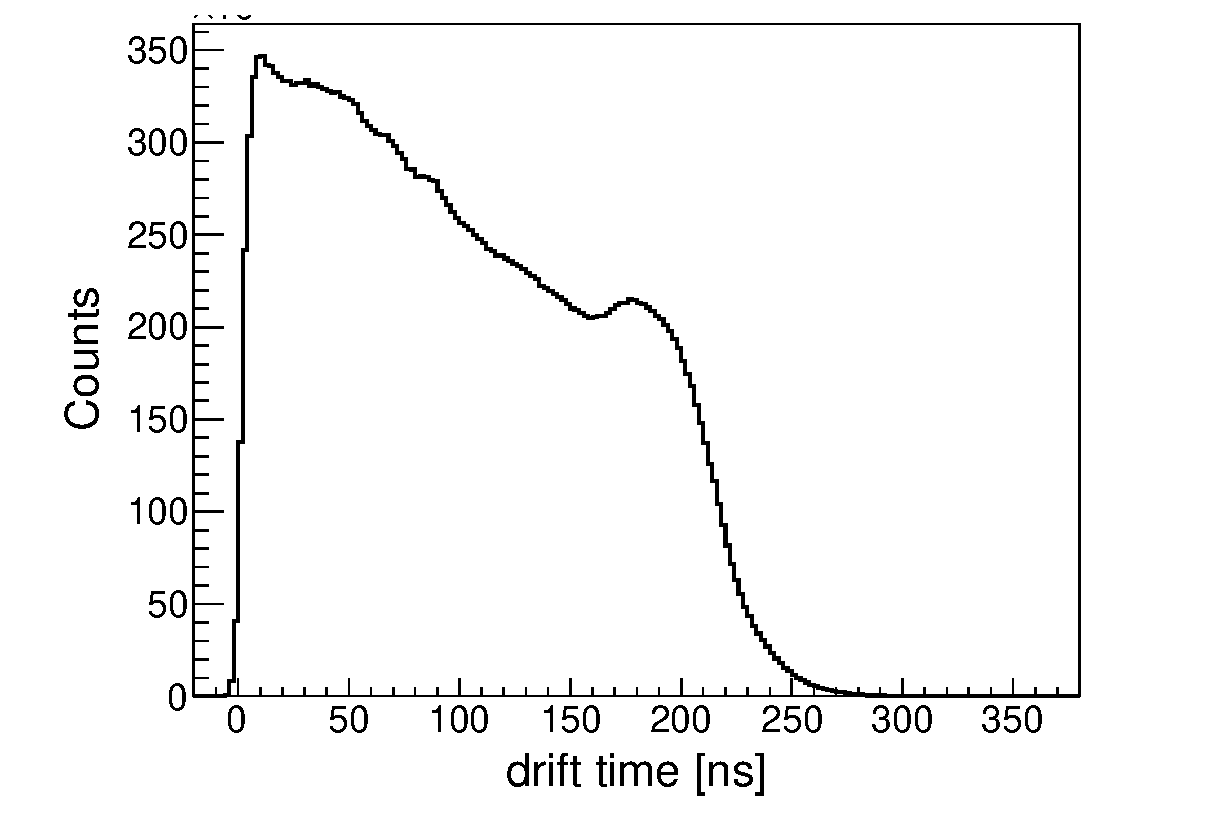
\includegraphics[width=6cm]{../pic/Run78/CDS/CDC_dl.eps}
    \end{minipage}

    \begin{minipage}{0.5\hsize}
      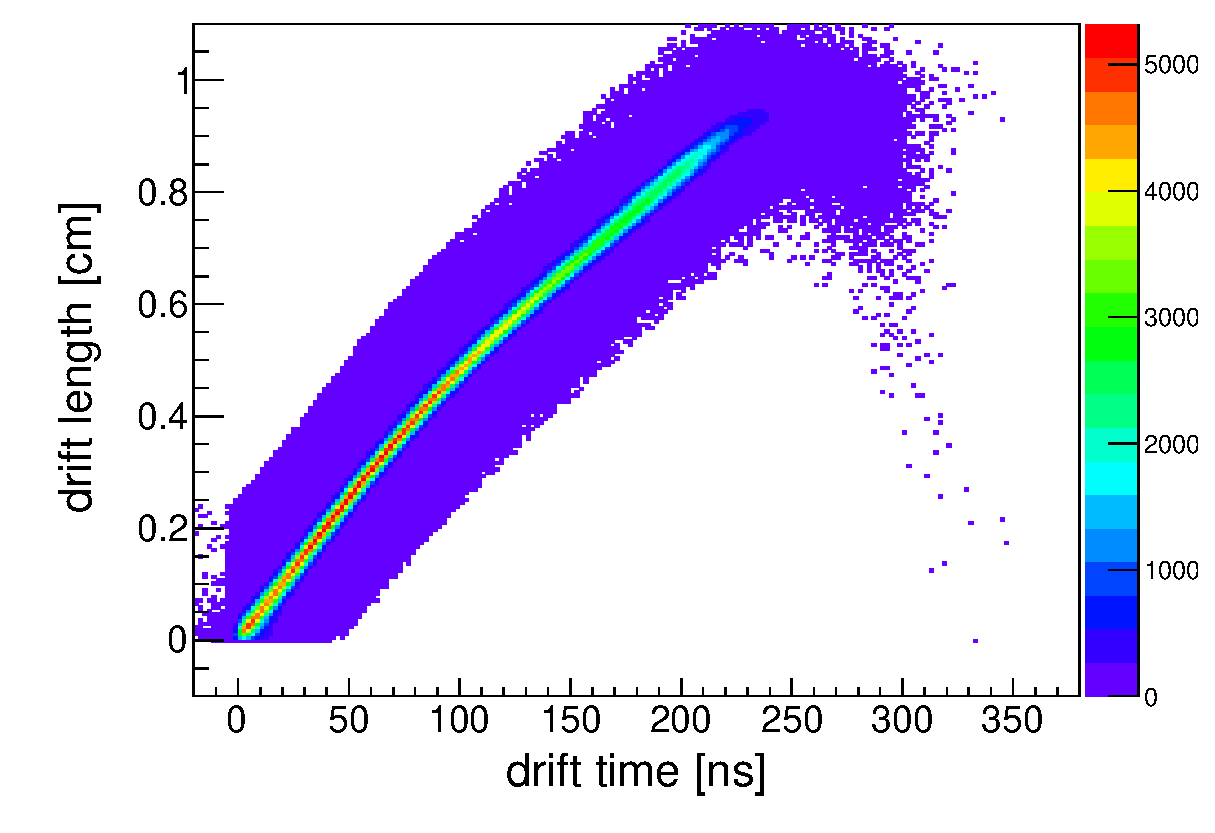
\includegraphics[width=6cm]{../pic/Run78/CDS/CDC_dl_dt.eps}
    \end{minipage}
  \end{tabular}
  \caption{
    Left figure shows drift time distribution of CDC.
    Right figure shows relation of drift time and drift length.
  }
  \label{fig:CDC_dl_dt}
\end{figure}

